\newpage
\section{Theoretische Grundlagen} \label{grundlange}

\subsection{Künstliche Intelligenz}

Die \ac{KI} ist ein Teilgebiet der Informatik und der Ingenieurswissenschaften. Innerhalb der Gesellschaft wird \ac{KI} als eine Simulation intelligenten 
menschlichen Denkens und Handelns aufgefasst.\footcite[][\pagef 2]{Mainzer.2019} 
Die KI-Forschung hat sich allerdings schon seit längerem von der Nachahmung menschlicher Intelligenz emanzipiert. 
Die Wissenschaft hat erkannt, dass es bessere Problemlösungsansätze gibt, als die Imitation des menschlichen Gehirns.
Vielmehr arbeitet die Forschung daran, Regeln und Prinzipien zu finden, die es einem Computer erlauben, die kogntiven Prozesse eines Menschen durch Berechnungsprozesse 
nachzubilden.~\footcite[\vglf][\pagef 11]{Lenzen.2020}

Moderne KI-Projekte sind eine Kooperation der Forschungsgebiete der Informatik, der Ingenieurskünste, der Mathematik, der Psychologie, der Biologie, der Linguistik,
der Neurowissenschaften, der Philosophie und der Ethnologie.
Die daraus hervorgehenden Systeme können z. B. Sätze analysieren und Fragen zum Inhalt eines Textes beantworten, indem sie Sprache verschriftlichen.
Auch sind sie in der Lage Bilder zu erkennen, diese zu analysieren und auf dieser Grundlage eigenständige Werke zu erschaffen.
Prominente Beispiele für solche System sind \enquote{ChatGPT} und \enquote{DALL·E2}.~\footcite[\vglf][\pagef 11]{Lenzen.2020}
Den Systemen stehen sehr große Mengen an Daten zur Verfügung, die durch sie auf erkennbare Muster durchsucht werden. So können diese die Auswirkung einer Entscheidung im Voraus 
berechnen und die Menschen so bei Entscheidungen unterstützen.~\footcite[\vglf][]{Lenzen.2020}

\ac{KI} kann in \enquote{starke} und \enquote{schwache} \ac{KI} kategorisiert werden. Dabei wäre eine starke \ac{KI} etwa eine Maschine,
welche eine ähnliche Intelligenz und Flexibilität wie ein Mensch besitzt. Eine schwache \ac{KI} hingegen ist ein System, welches nur eine Aufgabe besitzt, wie bspw. das Übersetzen.
Diese Kategorie bildet den größten Teil der KI-Forschung und -Produktentwicklung.~\footcite[\vglf][]{Lenzen.2020}

Bei \ac{KI}-Systemen im Allgemeinen besteht aber die Herausforderung zu entscheiden, ab wann diese als intelligent gelten, da es keine klare Definition des Wortes \enquote{Intelligenz} gibt.
Oft wird der Mensch als Maßstab für Definitionsansätze verwendet. Die \ac{KI}, zum heutigen Stand, übertrifft den Menschen jedoch bei weitem auf einem speziellen Gebiet wie z.B. Schach spielen
oder, wie oben bereits erwähnt, in große Datenmengen, im Folgenden nur noch als Big Data bezeichnet, nach Mustern zu durchsuchen, da sie anders funktionieren als der menschliche Verstand.
Konsens bei dem Verständnis von Intelligenz ist aber, dass sie auf Flexibilität und Lernen beruht und mit der Fähigkeit, auf wechselnde Anforderungen zu reagieren und die eigene 
Verhaltensweise erfahrungsbasiert anzupassen.~\footcite[\vglf][\pagef 14]{Lenzen.2020} 

\begin{figure}[H]
    \centering
    \captionsetup{justification=centering}
    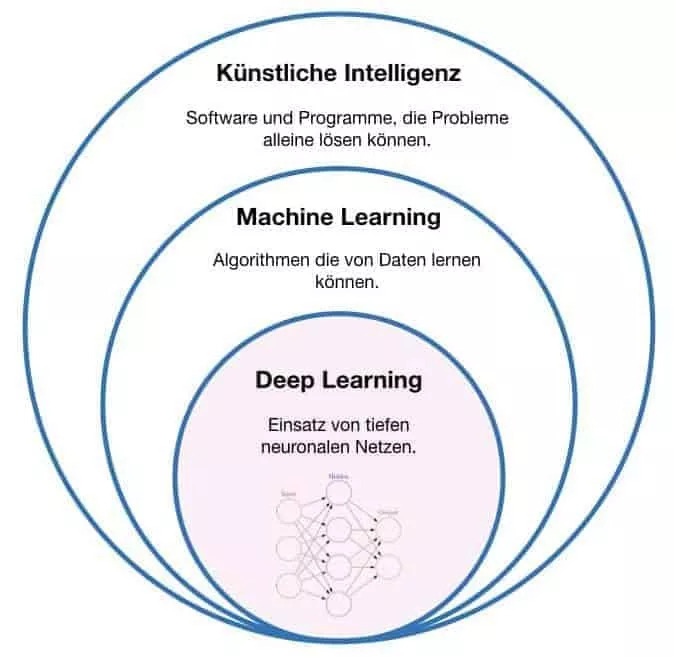
\includegraphics[width=0.8\textwidth]{deepL}
    \caption[Was ist Deep Learning?]{Was ist Deep Learning?\footnotemark}
    \label{fig:deepL}
\end{figure}
\footnotetext{\cite[\vglf][]{DeepLearning}}

Damit \ac{KI}-Systeme lernen, wird das sog. \enquote{maschinelle Lernen} eingesetzt. Wie in \autoref{fig:deepL} dargestellt ist, basiert dieses Verfahren auf Algorithmen, die von Daten lernen können. Tiefergreifend kommt dabei das 
sog. \enquote{Deep Learning}-Verfahren zum Einsatz, welches auf künstlichen neuronalen Netzen basiert.~\footcite[\vglf][]{Lenzen.2020}
Im Zuge der Digitalisierung wird unsere analoge Welt für solche informationsverarbeitenden Systeme in Form von Big Data lesbar gemacht und als Lernquelle zur Verfügung gestellt.
Gleichwohl bleiben die \ac{KI}-Systeme hoch spezialisiert und können sich nicht mit der flexiblen Intelligenz der Menschen messen. Um diese Hürde zu überwinden, nähert sich die 
aktuelle \ac{KI}-Forschung wieder an die Neurowissenschaft und der menschlichen Kognition an.~\footcite[\vglf][\pagef 18]{Lenzen.2020}

\subsection{Maschinelles lernen}

Eine manuelle Erstellung von Regeln und Wissenspräsentationen für die Verarbeitung durch \ac{KI}-Systeme, stellt einen hohen Aufwand mit nur einem begrenzten Nutzen dar.~\footcite[\vglf][\pagef 4]{Matzka.2021}
Um diesen Vorgang zu optimieren, werden nach Algorithmen und Techniken geforscht, die es \ac{KI}-Systemen ermöglichen selbständig allgemeingültige Regeln zu abstrahieren, in dem es selbständig Muster, aus einem ihm zur Verfügung stehenden
Datensatz, erkennt. Dies soll die Systeme befähigen, Vorhersagen oder Entscheidungen zu treffen, ohne explizit dafür programmiert worden zu sein. Dieser Vorgang nennt sich \ac{ML}.
Die zur Verfügung gestellten Datensätze werden auch als Trainingsdaten bezeichnet. Grundsätzlich bestehen sie aus Eingabeinformationen (Merkmalen) und Ausgabewerten (Labels oder Zielvariablen).
Besonders die Mustererkennung im hochdimensionalen Raum, durch gleichzeitige Berücksichtigung von hunderten oder tausenden Merkmalen, macht das \ac{ML} außergewöhnlich leistungsstark. Im Vergleich dazu ist es für einen Menschen
schon schwierig, drei- bis vierdimensionale Sachverhalte zu erfassen.~\footcite[\vglf][\pagef 5]{Matzka.2021}

Es existieren unterschiedlichen Arten des \ac{ML}. Beim überwachten Lernen werden dem System, wie bereits oben erwähnt, Trainingsdaten mit bekannten Eingaben und Ausgaben bereitgestellt. Daraus lernt 
das System über eine Abbildungsfunktion, neue Eingaben für die Ausgaben abzubilden.~\footcite[\vglf][\pagef 189]{Plaue.2021} Bei der Methodik des unüberwachten Lernens werden dem System nur Eingabedaten dargeboten und es wird erwartet,
dass es von selbst Muster und Strukturen in den Daten erkennt.~\footcite[\vglf][\pagef 255]{Plaue.2021} 
Das bestärkende Lernen basiert auf der positiven oder negativen Rückmeldung auf eine bestimmte Aktion. 
Ziel ist es, dass das \ac{KI}-System auf der Grundlage der gemachten \enquote{Lernerfahrung} selbständig Vorhersagen und Entscheidungen trifft. 
Die Qualität dieser sind abhängig von der Qualität und Repräsentativität der verwendeten Daten. Auch muss der Mensch hier weiterhin evaluieren, ob die getroffenen Vorhersagen oder Entscheidungen
zuverlässig und vertrauenswürdig sind.

\ac{KI}-Systeme mit \ac{ML} werden besonders in Bereichen mit Aufgabengebieten eingesetzt, in denen Menschen Schwierigkeiten haben, diese zu lösen. Die menschliche Intelligenz wird dabei nicht ersetzt
oder simuliert, sondern komplementiert.~\footcite[\vglf][\pagef 5]{Matzka.2021}


\subsection{Big Data}

Damit {KI}-Systeme lernen können, brauchen sie sehr große Datenmengen, welche als Big Data bezeichnet werden. Dabei handelt es sich um großen Datenmengen, die in unterschiedlichen Formaten auftreten
und in verschiedenen Quellen generiert wurden. Der Autor Ralf Huss definiert Big Data als Datenmengen, die zu groß, zu komplex oder zu schwach strukturiert sind oder sich zu schnell ändern, um mit herkömmlichen
Methoden analysiert zu werden.~\footcite[][\pagef 60]{Huss.2019} Darin liegt die große Bedeutung von Big Data, nämlich wertvolle Erkenntnisse und Muster aus Daten zu extrahieren,
bei denen herkömmliche Analysemethoden nicht ausreichen würden. Dabei können die Daten aus traditionellen Datenbanksystemen stammen oder in unstrukturierten Formaten wie Text, Audio, Video und Sensordaten vorliegen.~\footcite[\vglf][\pagef 7]{Fasel.2019}

Big Data besitzt drei Hauptcharakteristika, welche im Folgenden aufgezählt und kurz erklärt werden:

\begin{itemize}
    \item Volume - der Datenbestand bei Big Data kann enorme Ausmaße annehmen und liegt im Tera- (10\textsuperscript{12} Bytes) bis Zettabytebereich (10\textsuperscript{21} Bytes). 2008 wurden weltweit 10 Zettabytes (10\textsubscript{21} Bytes) verarbeitet.~\footcite[\vglf][\pagef 61]{Huss.2019}
    \item Variety - der Begriff bedeutet übersetzt Vielfalt. Strukturierte Daten aus z. B. Datenbanken, semi-strukturiete Daten wie z.B. Logdateien oder Sensordaten und unstrukturierte Daten wie z.B. Textdokumente, E-Mails und Multimediadateien, werden gespeichert.~\footcite[\vglf][\pagef 6]{Fasel.2019}
    \item Velocity - der entstehende Datenstrom (Data Stream) bei Big Data wird in Echtzeit generiert und muss von entsprechend schnellen Erfassungs-, Verarbeitungs- und Analysemethoden in Echtzeit erfasst und analysiert werden.~\footcite[\vglf][]{Fasel.2019}
\end{itemize}


In einigen Quellen werden noch weitere Charakteristika für Big Data definiert, welche ebenfalls im Folgenden aufgezählt und kurz erklärt werden: 

\begin{itemize}
    \item Value - der Wert des Unternehmens soll gesteigert werden~\footcite[\vglf][]{Fasel.2019}. Dabei ist nicht unbedingt allein der monetäre Wert gemeint. In Bezug auf die Daten muss geklärt werden,
    welche Erkenntnisse aus Ihnen abgeleitet werden können, um für das verarbeitende Unternehmen einen Mehrwert darzustellen. 
    \item Veracity - da die Qualität der Daten nicht per se bekannt sind, müssen spezielle Algorithmen eingesetzt werden, um die Qualität der Resultate bzw. die Plausibilität dieser zu evaluieren. Dabei garantiert
 ein größerer Datensatz keine bessere Aussagequalität~\footcite[\vglf][]{Fasel.2019}.
\end{itemize}

Die Herausforderungen bei Big Data umfassen vor allem die Datenerfassung, -speicherung, -verarbeitung und -analyse in angemessener Zeit, Datenschutz und Datensicherheit und insbesondere die Gewährleistung der 
Datenqualität. Um diese Herausforderungen zu bewältigen, müssen Technologien wie NoSQL-Datenbanken, Cloud-Computing und verteilte System eingesetzt werden.

Big Data hat das Potenzial einen erheblichen Mehrwert für Unternehmen, Organisationen, Forschungseinrichtungen und die Gesellschaft insgesamt zu schaffen, indem es Einblicke und Erkenntnisse liefert, 
die zuvor nicht möglich waren. Es ermöglicht, bessere Entscheidungen zu treffen, Effizienz und Produktivität zu steigern und Innovationen voranzutreiben.

\subsection{Datenschutzgrundverordnung}

Die \ac{DSGVO} wurde in ihrer jetzigen Form 2018 von der Europäischen Union verabschiedet und ist ein einheitlicher Rechtsrahmen mit dem ein verantwortungsbewusster Umgang
mit personenbezogenen Daten der Bürger der \ac{EU} sichergestellt wird.~\footcite[\vglf][\pagef 2]{Voigt.2018}
Die Verordnung stärkt vor allem die Rechte der Bürger bei der Verarbeitung ihrer personenbezogenen Daten z. B. durch Unternehmen. Personenbezogene Daten sind alle Daten, die einen Menschen
\enquote{identifizierbar} machen. Dabei reicht die bloße Möglichkeit der \enquote{Identifizierung} durch eine Kombination verschiedener Informationen, 
die für sich allein keinen Rückschluss 
auf den Betroffenen möglich gemacht hätten, aber es ermöglichen würden, um als personenbezogene Daten qualifiziert zu werden.~\footcite[\vglf][\pagef 14]{Voigt.2018}

Im Folgenden werden die wichtigsten Punkte der \ac{DSGVO} aufgeführt. Jeder \ac{EU}-Bürger hat das Recht zu erfahren, welche Daten über ihn gesammelt werden, warum diese Daten gesammelt werden, wie sie verwendet werden und an wen diese Daten übermittelt werden. 
Dies wird auch als Auskunftsrecht bezeichnet. Weiterführend können diese Daten durch den Bürger
berichtigt werden, falls diese falsch oder unvollständig sind. Er hat ein Recht auf diese Berichtigung aber auch das Recht seine Daten löschen zu lassen. Ebenfalls ist es ihm möglich die 
Verarbeitung durch das Unternehmen einzuschränken oder dieser im gesamten zu widersprechen.~\footcite[\vglf][\pagef 200]{Voigt.2018} Des Weiteren hat er das Recht der Datenübertragbarkeit. Hierbei müssen die Daten der
betroffenen Person in einem gängigen maschinenlesbaren Format übermittelt werden oder diese einem anderen Unternehmen bereitstellen.
Personenbezogene Daten dürfen nicht ohne die Einwilligung der betroffenen Person erhoben oder verarbeitet werden. Dabei muss die Einwilligung freiwillig, spezifisch, informiert und
unmissverständlich sein.
Unternehmen müssen \enquote{Datenpannen}, z. B. die Offenlegung von personenbezogenen Daten, innerhalb von 72 Stunden an eine Datenschutzbehörde melden.~\footcite[\vglf][\pagef 86]{Voigt.2018}
Die \ac{DSGVO} ist noch deutlich umfangreicher und hat beträchtliche Auswirkung auf Unternehmen, besonders solche, die große Mengen an personenbezogenen Daten sammeln und verarbeiten.
Sie dienen vor allem dem Schutz der Privatsphäre der \ac{EU}-Bürger.
Verstöße gegen die DSGVO können zu erheblichen Strafen führen. Unternehmen sind daher angehalten, ihre Datenverarbeitungsprozesse sorgfältig zu prüfen und zu verwalten.~\footcite[\vglf][\pagef 85]{Voigt.2018}

